\documentclass[a4paper, 11pt]{article}
\usepackage[left=3cm, top=3cm, right=2cm, bottom=2cm]{geometry}
%pacote que define as margens
\usepackage{helvet} % carrega o documento com Fonte ARIAL
\renewcommand{\familydefault}{\sfdefault} % define a fonte ARIAL como padrão do texto
\usepackage[utf8]{inputenc} %pacote que normaliza a acentuação
\usepackage[T1]{fontenc}
\usepackage[brazil]{babel} %pacote que define o idioma
\usepackage{graphicx} %pacote que permite a inserção de imagens
\pagestyle{myheadings} %pacote que define o cabeçalho com o número de página no canto superior direito
\usepackage{setspace} %pacote que permite especificar o espaçamento entre linhas no documento
\usepackage{indentfirst} %pacote que faz indentação na primeira linha do parágrafo
\setlength{\parindent}{1cm} %pacote que define o tamanho da indentação
\usepackage{float} %Pacote que permite tabelas flutuarem em qualquer posição
% \usepackage[alf,abnt-repeated-title-omit=yes,abnt-emphasize=bf,abnt-etal-list=0]{abntex2cite} %define os parâmetros necessários para as referências e citações de acordo com a ABNT
\usepackage{amsthm}
\usepackage{amsfonts}
\usepackage{subcaption} % Pacote que permite que imagens possam ser inseridas em composições de imagens lado a lado com o \subfigure
\usepackage{amssymb} %4 Pacotes responsáveis pela formatação matemática
\usepackage{rotating} %permite que textos, figuras e tabelas possam ser rotacionados
\usepackage{array}    % permite e vetorização de tabelas
\usepackage{longtable} % permite a elaboração de tabelas complexas
\usepackage{colortbl} % permite a utilização de paletas de cores
\usepackage{tikz} % criação de objetos vetoriais
\usetikzlibrary{shapes, arrows.meta, positioning}
\usepackage{pdflscape} % permite alterar o estilo da pagina entre portrato e paisagem
\usepackage{hyperref}
\hypersetup{
colorlinks=true,
linkcolor=black, % alterado para black, antes darkblue por bug
filecolor=magenta,
urlcolor=blue,
citecolor=black,
pdftitle={mybib},
pdfpagemode=FullScreen
}
\usepackage{sectsty}
\sectionfont{\fontsize{12}{12}\selectfont}
\subsectionfont{\fontsize{12}{12}\selectfont}
\subsubsectionfont{\fontsize{12}{12}\selectfont}
\usepackage{url}
\usepackage{pgfplots}
%\usepackage[table,xcdraw]{xcolor}
%\usepackage[brazilian,hyperpageref]{backref}	% Paginas com as citações na bibl
%\usepackage[num,overcite]{abntex2cite} % Citações padrão ABNT
%\usepackage{cite}
%\usepackage{pgfgantt}  % gera gantt em latex
\usepackage{acronym} 
%\usepackage[acronym]{glossaries} % cria glossário de siglas
%\makeglossaries
\usepackage[most]{tcolorbox}
\usepackage{listings}        % Para listar códigos
\lstset{
	inputencoding=utf8,
	extendedchars=true,
	literate={á}{{\'a}}1 {é}{{\'e}}1 {í}{{\'i}}1 {ó}{{\'o}}1 {ú}{{\'u}}1
	{Á}{{\'A}}1 {É}{{\'E}}1 {Í}{{\'I}}1 {Ó}{{\'O}}1 {Ú}{{\'U}}1
	{à}{{\`a}}1 {è}{{\`e}}1 {ì}{{\`i}}1 {ò}{{\`o}}1 {ù}{{\`u}}1
	{À}{{\`A}}1 {È}{{\`E}}1 {Ì}{{\`I}}1 {Ò}{{\`O}}1 {Ù}{{\`U}}1
	{ã}{{\~a}}1 {õ}{{\~o}}1 {Ã}{{\~A}}1 {Õ}{{\~O}}1
	{â}{{\^a}}1 {ê}{{\^e}}1 {î}{{\^i}}1 {ô}{{\^o}}1 {û}{{\^u}}1
	{Â}{{\^A}}1 {Ê}{{\^E}}1 {Î}{{\^I}}1 {Ô}{{\^O}}1 {Û}{{\^U}}1
	{ç}{{\c{c}}}1 {Ç}{{\c{C}}}1
}

%\usepackage{xcolor}

\definecolor{codegreen}{rgb}{0,0.6,0}
\definecolor{codegray}{rgb}{0.5,0.5,0.5}
\definecolor{codepurple}{rgb}{0.58,0,0.82}
\definecolor{backcolour}{rgb}{0.95,0.95,0.92}

\lstdefinestyle{mystyle}{
	backgroundcolor=\color{backcolour},   
	commentstyle=\color{codegreen},
	keywordstyle=\color{magenta},
	numberstyle=\tiny\color{codegray},
	stringstyle=\color{codepurple},
	basicstyle=\ttfamily\footnotesize,
	breakatwhitespace=false,         
	breaklines=true,                 
	captionpos=b,                    
	keepspaces=true,                 
	numbers=left,                    
	numbersep=5pt,                  
	showspaces=false,                
	showstringspaces=false,
	showtabs=false,                  
	tabsize=2
}

\lstset{style=mystyle}


\begin{document}  
    % Deve conter o título do trabalho, nome do autor, nome da instituição, curso, orientador, local e ano. A capa deve seguir as normas da instituição para formatação (ABNT ou outra específica).
	\thispagestyle{empty}

\begin{center}
	\begin{figure}[h]
  \centering
		
\includegraphics[width=0.21\linewidth]{imagens/ufpa.png}
		\label{fig:ufpa}
	\end{figure}
	
	
	\vspace{1cm}
	\large \uppercase{UNIVERSIDADE FEDERAL DO PARÁ}\\
	\large \uppercase{INSTITUTO DE TECNOLOGIA}\\
	\large \uppercase{BACHARELADO EM ENGENHARIA MECÂNICA}\\
	\vspace{6cm}
	\large \uppercase{CINEMÁTICA DOS MECANISMOS}\\
	\vspace{1cm}
	\large \uppercase {AVALIAÇÃO FINAL: LISTA DE EXERCÍCIOS 1} \\
	\vspace{7cm}
	\large {BELÉM/PA \\ 2025}

 \newpage
 \thispagestyle{empty}
 \large \uppercase{alan henrique pereira miranda - 202102140072}\\
 \vspace{5cm}
	\large \uppercase{CINEMÁTICA DOS MECANISMOS}\\
\vspace{1cm}
	\large \uppercase {AVALIAÇÃO FINAL: LISTA DE EXERCÍCIOS 1} \\
 \vspace{1cm}
 \singlespacing
 \hspace{8cm} % posicionando a caixa de texto
 \begin{minipage}{7cm}
	Atividade referente à primeira avaliação da disciplina Cinemática dos Mecanismos, lecionada na Universidade Federal do Pará. \\
	
	Profa. Dr.: Fábio Seturbal
	\vspace{1cm}
	
	Belém-PA 15 de janeiro de 2025
	\vspace{4cm}
\end{minipage}

\onehalfspacing
\begin{center}
	
	EXAMINADOR\\
	\vspace{3cm}
	\rule{10cm}{0.15mm} \\
	Profa. Dr.: Fábio Seturbal\\
	Universidade Federal do Pará - UFPA
\end{center}
\newpage

\begin{center}
    % BLOCO DE FIGURAS
    \thispagestyle{empty}
	\listoffigures
	\newpage
    % SUMARIO
    \thispagestyle{empty}
    \tableofcontents

\end{center}

\newpage
\thispagestyle{empty}
	
\end{center}
    % Resumo, dedicatórias etc (elementos pré extuais)


    % elementos textuais
    % -> introdução: Conteúdo: Apresenta o tema do trabalho, o problema a ser investigado, os objetivos gerais e específicos, a justificativa para a realização do estudo e uma breve descrição da estrutura do documento. Deve contextualizar o leitor sobre a relevância do trabalho.
	\section{Introdução}

Por volta de 20.000 aC. o homem já utilizava uma espécie de dispositivo que viabilizava a troca de calor, conhecido como panela de cozinhar. Arquimedes de Siracusa, por volta de 212 A.C., criou o primeiro dispositivo de calor destinado ao uso comercial e público, o canhão a vapor. Heron, em 120 A.C., criou outro dispositivo, a esfera gigante. Entretanto, somente em 1763 o trocador de calor foi lançado, com a criação da máquina a vapor de James Watt; \cite{abdallah_2018_multi}

Atualmente, os trocadores de calor apresentam grande importância por fornecer Alta eficiência térmica no processo de transferência de calor, baixo custo de instalação, alta performance, com baixo volume retido, fácil desmontagem para manutenção e, por ser um equipamento geralmente desmontável, permite o ajuste da capacidade do trocador adicionando ou removendo placas do equipamento.\cite{abdallah_2018_multi}

Por definição, os trocadores de calor são equipamentos responsáveis por realizar troca térmica entre dois ou mais fluidos a diferentes temperaturas, podendo ou não ocorrer mudança de fase dos fluidos. Adota-se trocador de calor ao equipamento que não promove a mudança de fase dos fluidos, enquanto os que ocorrem essa alteração recebem nomes específicos, como evaporadores, condensadores, refervedores ou vaporizadores. Dentre os variados campos de aplicação desses equipamentos estão indústrias de processo, química e alimentícia, resfriamento e/ou aquecimento de ambientes, condicionamento de ar, recuperação de calor, produção de energia, radiadores de automóveis e veículos espaciais.\cite{abdallah_2018_multi}
Os trocadores de calor possuem configurações dos mais variados tipos para as mais variadas aplicações. O trocador de calor que será dimensionado e selecionado neste trabalho será o do tipo casco e tubo, cuja configuração geral segue exemplificada na figura \ref{fig:fig1}: \cite{abdallah_2018_multi, incase_2022_trocador}
\\
\begin{figure}[h]
	\centering
	\caption{Trocador de calor de casco e tubo}
	\label{fig:fig1}
	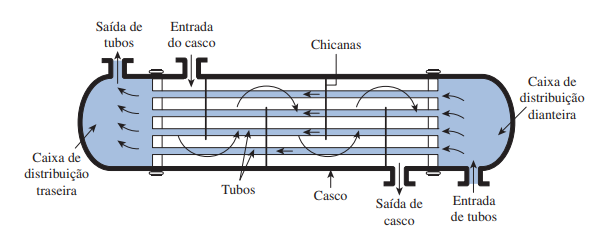
\includegraphics[width=1\linewidth]{imagens/fig1}
	
	\text{Fonte: \cite{incase_2022_trocador}}
\end{figure}

\subsection{Tipos principais de trocadores de calor e configuração de escoamentos}
Os dois principais tipos de trocadores de calor encontrados nas aplicações rotineiras são os seguintes:
\begin{itemize}
	\item Casco e Tubo;
	\item Tubo duplo;
	\item Placas Paralelas;
\end{itemize}

O trocador de casco e tubos é o mais utilizado na indústria de refino de petróleo, uma vez que possui amplas faixas de vazão, temperatura e pressão \cite{orgeda_2020_trocadores}. Em geral, é o único que pode ser aplicado em processos que necessitam de grandes áreas de troca de calor, acima de \(5000m^2\), pressões acima de \(30bar\) e temperaturas superiores a \(260^oC\) \cite{orgeda_2020_trocadores}. Aliado a isso, pode operar com líquidos, gases ou vapores, como condensador ou vaporizador, em posição horizontal ou vertical, de acordo com as necessidades operacionais a serem determinadas \cite{orgeda_2020_trocadores}. 

\begin{figure}[h]
	\centering
	\caption{Trocador de calor com múltiplos tubos internos}
	\label{fig:fig2}
	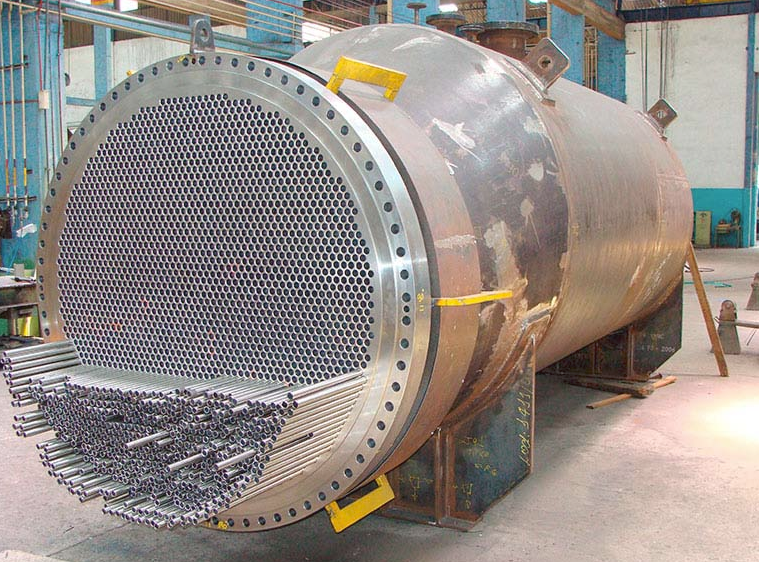
\includegraphics[width=.7\linewidth]{imagens/fig2}
	
	\text{Fonte: \cite{incase_2022_trocador}}
\end{figure}
O modelo mais simples de trocador de calor é o chamado trocador de tubo duplo, que consiste essencialmente em dois tubos concêntricos, em que um dos fluidos escoa pelo tubo de diâmetro menor e o outro escoa pelo espaço anular entre os dois tubos. Geralmente, este tipo de trocador apresenta dois trechos retos com conexões nas extremidades dos tubos.

\begin{figure}[h]
	\centering
	\caption{Esquemático: Trocador de tubo duplo}
	\label{fig:fig3}
	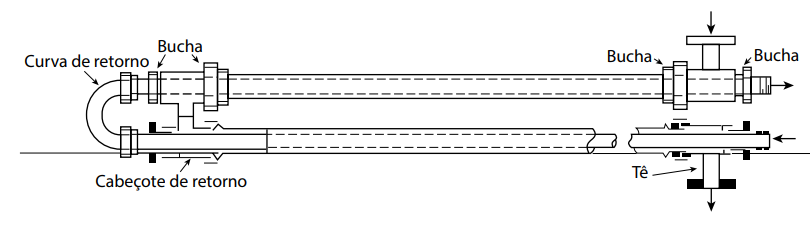
\includegraphics[width=.8\linewidth]{imagens/fig3}
	
	\text{Fonte: \cite{orgeda_2020_trocadores}}
\end{figure}

O fluxo do escoamento dos fluidos que exercerão a troca térmica ao longo dos componentes do trocador de calor em questão define papel crucial no desempenho do trocador de calor. Em suma, os perfis de temperatura de ambos os fluidos que trocam calor apresentam perfis diferentes em função da direção dos escoamentos. Em geral, são utilizados dois tipos de escoamentos em trocadores de calor: escoamento paralelo e contracorrente.

 Para o escoamento paralelo, as temperaturas dos dois fluidos tendem a se aproximar e a diferença de temperatura ao longo do trocador diminui significativamente. De outra forma, para o escoamento contracorrente, o fluido frio pode sair do equipamento mais quente do que o próprio fluido quente sai, e as diferenças de temperatura entre os dois fluidos ao longo do trocador apresentam menor variação \cite{cengel_2012_transferencia}. A figura \ref{fig:fig4} representa de forma simplificada estas duas situações:
 
 
 \begin{figure}[h]
 	\centering
 	\caption{Arranjos de escoamento em trocadores de calor e seus perfis de temperatura associados.}
 	\label{fig:fig4}
 	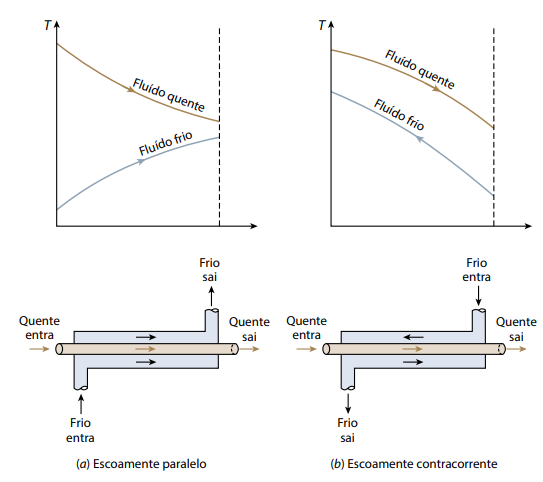
\includegraphics[width=.7\linewidth]{imagens/fig4}
 	
 	\text{Fonte: \cite{cengel_2012_transferencia}}
 \end{figure}
 
 

	% SECÇÃO FUNDAMENTOS
	\section{Questão 12-9}

\begin{figure}[H]
	\centering
	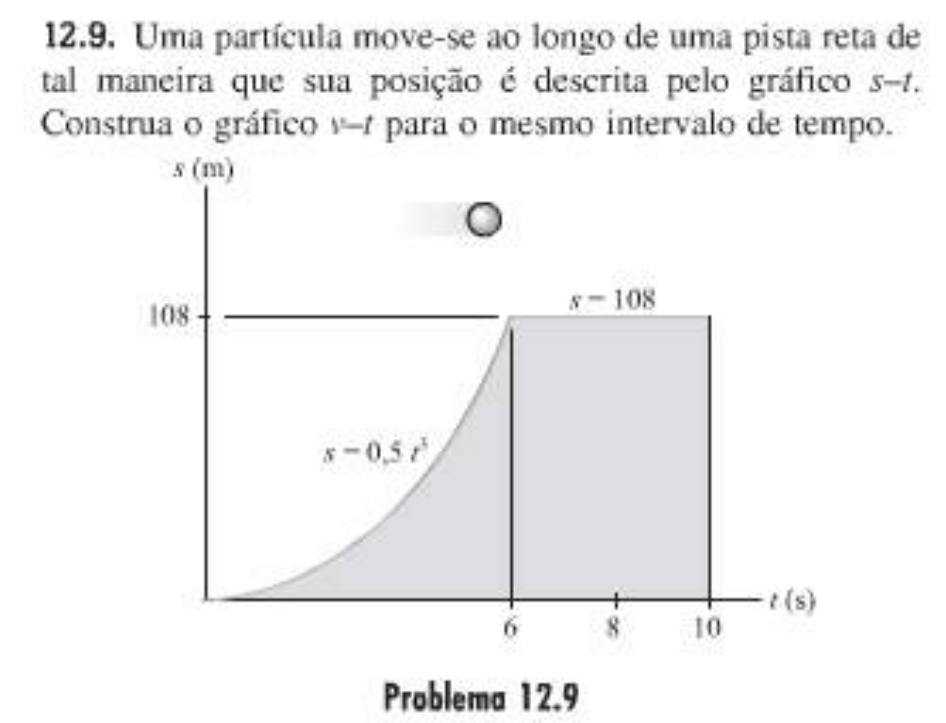
\includegraphics[width=.7\linewidth]{fundamentais/12-9.png}
	\caption{Comando da questão 12-9}\label{fig:q12-9}
\end{figure}

Nesta questão, analisamos a função da posição \(s(t)\) e determinamos a expressão para a velocidade \(v(t)\) em diferentes intervalos de tempo. Além disso, apresentamos os resultados em forma gráfica.

\subsection*{Função da Posição \(s(t)\)}
A função da posição \(s(t)\) é definida por:
\[
s(t) = 
\begin{cases} 
0.5t^2 & \text{se } 0 <  t \leq 6, \\
108 & \text{se } 10 \geq t > 6.
\end{cases}
\]

\subsection*{Cálculo da Velocidade \(v(t)\)}
A velocidade \(v(t)\) é obtida pela derivada da posição \(s(t)\) em relação ao tempo \(t\). Para \(t \leq 6\), temos:
\[
s(t) = 0.5t^2 \implies v(t) = \frac{d}{dt}s(t) = t.
\]

Para \(t > 6\), como \(s(t)\) é constante (\(s(t) = 108\)), a velocidade é:
\[
v(t) = 0.
\]

Portanto, a velocidade \(v(t)\) é definida por:
\[
v(t) = 
\begin{cases} 
t & \text{se } t \leq 6, \\
0 & \text{se } t > 6.
\end{cases}
\]

\subsection*{Dados Gerados}
Os dados de tempo (\(t\)), posição (\(s(t)\)), e velocidade (\(v(t)\)) foram gerados e organizados para análise. A tabela a seguir ilustra os valores calculados (valores exemplares):

\begin{table}[H]
    \centering
    \begin{tabular}{|c|c|c|}
        \hline
        \textbf{Tempo (s)} & \textbf{Posição (m)} & \textbf{Velocidade (m/s)} \\
        \hline
        0.0 & 0.0 & 0.0 \\
        1.0 & 0.5 & 1.0 \\
        2.0 & 2.0 & 2.0 \\
        \vdots & \vdots & \vdots \\
        6.0 & 18.0 & 6.0 \\
        7.0 & 108.0 & 0.0 \\
        8.0 & 108.0 & 0.0 \\
        \hline
    \end{tabular}
    \caption{Dados de posição e velocidade em função do tempo.}
\end{table}

\subsection*{Gráfico de Velocidade \(v(t)\)}
A função \(v(t)\) foi representada graficamente. O eixo \(x\) corresponde ao tempo (\(t\)), enquanto o eixo \(y\) corresponde à velocidade (\(v(t)\)). Uma linha vertical foi traçada em \(t = 6\), indicando a mudança no comportamento da função.

\begin{figure}[H]
    \centering
    \begin{tikzpicture}
    \begin{axis}[
        width=12cm, height=8cm,
        xlabel={Tempo (s)},
        ylabel={Velocidade (m/s)},
        grid=major,
        legend pos=north west,
        title={Gráfico Velocidade x Tempo}
    ]
        \addplot[domain=0:6, samples=100, blue, thick] {x};
        \addplot[domain=6:10, samples=100, blue, thick] {0};
        \addplot[dashed, red, thick] coordinates {(6, 0) (6, 6)};
        \legend{$v(t)$, $t = 6$ s (mudança)};
    \end{axis}
    \end{tikzpicture}
    \caption{Gráfico da função velocidade \(v(t)\).}\label{fig:figure}
\end{figure}

\subsection*{Resultados Finais}
\begin{itemize}
    \item Função da posição:
    \[
    s(t) = 
    \begin{cases} 
    0.5t^2 & \text{se } t \leq 6, \\
    108 & \text{se } t > 6.
    \end{cases}
    \]
    \item Função da velocidade:
    \[
    v(t) = 
    \begin{cases} 
    t & \text{se } t \leq 6, \\
    0 & \text{se } t > 6.
    \end{cases}
    \]
\end{itemize}

	\newpage
\section{Questão 12-15}


\begin{figure}[H]
	\centering
	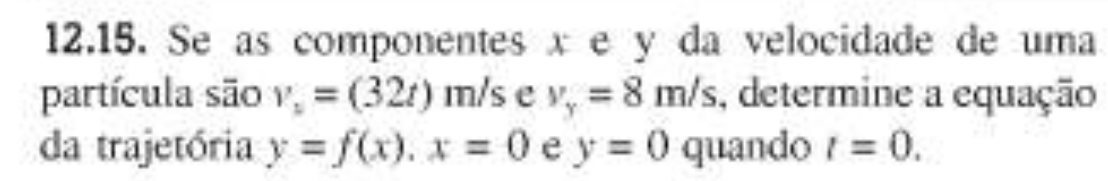
\includegraphics[width=.7\linewidth]{fundamentais/12-15.png}
	\caption{Comando da questão 12-15.}\label{fig:q12-15}
\end{figure}


Nesta questão, determinamos as equações paramétricas das posições \(x(t)\) e \(y(t)\), bem como a relação cartesiana entre as coordenadas \(x\) e \(y\), com base nos componentes da velocidade. A seguir, detalhamos o equacionamento.

\subsection*{Definição das Variáveis e Componentes de Velocidade}
As variáveis e os componentes da velocidade são definidos como:
\[
v_x = 32t, \quad v_y = 8,
\]
onde:
\begin{itemize}
    \item \(t\) representa o tempo;
    \item \(x\) e \(y\) representam as coordenadas no espaço.
\end{itemize}

\subsection*{Integração para Determinar as Posições em Função do Tempo}
A posição na direção \(x\) é obtida pela integração de \(v_x\):
\[
x(t) = \int v_x \, dt = \int 32t \, dt = 16t^2 + C_1.
\]

A posição na direção \(y\) é obtida pela integração de \(v_y\):
\[
y(t) = \int v_y \, dt = \int 8 \, dt = 8t + C_2.
\]

\subsection*{Determinação das Constantes de Integração}
Utilizando as condições iniciais:
\[
x(0) = 0 \quad \text{e} \quad y(0) = 0,
\]
determinamos as constantes \(C_1\) e \(C_2\):
\[
x(0) = 16(0)^2 + C_1 \implies C_1 = 0,
\]
\[
y(0) = 8(0) + C_2 \implies C_2 = 0.
\]

Substituindo as constantes nas equações, obtemos:
\[
x(t) = 16t^2, \quad y(t) = 8t.
\]

\subsection*{Eliminação de \(t\) para Determinar \(y\) em Função de \(x\)}
Da equação de \(x(t)\), resolvemos \(t\) em função de \(x\):
\[
x(t) = 16t^2 \implies t = \sqrt{\frac{x}{16}} = \frac{\sqrt{x}}{4}.
\]

Substituindo \(t\) na equação de \(y(t)\), obtemos:
\[
y = 8t = 8 \cdot \frac{\sqrt{x}}{4} = 2\sqrt{x}.
\]

Portanto, a equação cartesiana entre \(x\) e \(y\) é:
\[
y(x) = 2\sqrt{x}.
\]

\subsection*{Resultados Finais}
\begin{itemize}
    \item Equações paramétricas:
    \[
    x(t) = 16t^2, \quad y(t) = 8t.
    \]
    \item Relação cartesiana entre \(x\) e \(y\):
    \[
    y(x) = 2\sqrt{x}.
    \]
\end{itemize}

	\section{Questão 12-17}

Nesta questão, analisamos o movimento de uma partícula cuja trajetória é definida por uma parábola \(y^2 = 4x\), com a posição em \(x\) dada como função do tempo \(t\). Determinamos as velocidades, acelerações e suas intensidades, bem como os valores numéricos no instante \(t = 0.5 \, \text{s}\).

\subsection*{Equação da Trajetória}
A equação da trajetória da partícula é definida como:
\[
y^2 = 4x,
\]
onde a posição \(x\) é dada por:
\[
x(t) = 4t^4.
\]

\subsection*{Cálculo das Derivadas para \(x\)}
A velocidade na direção \(x\) é obtida pela derivada de \(x(t)\) em relação ao tempo \(t\):
\[
v_x = \frac{dx}{dt} = \frac{d}{dt}\left(4t^4\right) = 16t^3.
\]

A aceleração na direção \(x\) é a derivada de \(v_x\):
\[
a_x = \frac{dv_x}{dt} = \frac{d}{dt}\left(16t^3\right) = 48t^2.
\]

\subsection*{Substituição de \(x\) na Equação da Trajetória}
Substituímos \(x(t)\) na equação da trajetória para encontrar \(y(t)\):
\[
y^2 = 4x \implies y^2 = 4(4t^4) \implies y = 4t^2.
\]

\subsection*{Cálculo das Derivadas para \(y\)}
A velocidade na direção \(y\) é:
\[
v_y = \frac{dy}{dt} = \frac{d}{dt}\left(4t^2\right) = 8t.
\]

A aceleração na direção \(y\) é:
\[
a_y = \frac{dv_y}{dt} = \frac{d}{dt}\left(8t\right) = 8.
\]

\subsection*{Intensidade da Velocidade}
A intensidade da velocidade é dada por:
\[
|\vec{v}| = \sqrt{v_x^2 + v_y^2}.
\]

Substituindo \(v_x\) e \(v_y\):
\[
|\vec{v}| = \sqrt{(16t^3)^2 + (8t)^2} = \sqrt{256t^6 + 64t^2}.
\]

\subsection*{Intensidade da Aceleração}
A intensidade da aceleração é dada por:
\[
|\vec{a}| = \sqrt{a_x^2 + a_y^2}.
\]

Substituindo \(a_x\) e \(a_y\):
\[
|\vec{a}| = \sqrt{(48t^2)^2 + (8)^2} = \sqrt{2304t^4 + 64}.
\]

\subsection*{Cálculos no Instante \(t = 0.5 \, \text{s}\)}
Substituímos \(t = 0.5 \, \text{s}\) nas equações para obter os valores numéricos:
\begin{itemize}
    \item Velocidade em \(x\): 
    \[
    v_x = 16t^3 \implies v_x = 16(0.5)^3 = 2.0 \, \text{m/s}.
    \]
    \item Velocidade em \(y\): 
    \[
    v_y = 8t \implies v_y = 8(0.5) = 4.0 \, \text{m/s}.
    \]
    \item Intensidade da velocidade:
    \[
    |\vec{v}| = \sqrt{256(0.5)^6 + 64(0.5)^2} \implies |\vec{v}| \approx 4.47 \, \text{m/s}.
    \]
    \item Intensidade da aceleração:
    \[
    |\vec{a}| = \sqrt{2304(0.5)^4 + 64} \implies |\vec{a}| \approx 34.06 \, \text{m/s}^2.
    \]
\end{itemize}

\subsection*{Resultados Finais}
\begin{itemize}
    \item Equações paramétricas:
    \[
    x(t) = 4t^4, \quad y(t) = 4t^2.
    \]
    \item Velocidade:
    \[
    v_x = 16t^3, \quad v_y = 8t.
    \]
    \item Aceleração:
    \[
    a_x = 48t^2, \quad a_y = 8.
    \]
    \item Intensidades:
    \[
    |\vec{v}| = \sqrt{256t^6 + 64t^2}, \quad |\vec{a}| = \sqrt{2304t^4 + 64}.
    \]
    \item Valores no instante \(t = 0.5 \, \text{s}\):
    \begin{itemize}
        \item \(v_x = 2.0 \, \text{m/s}\),
        \item \(v_y = 4.0 \, \text{m/s}\),
        \item \(|\vec{v}| \approx 4.47 \, \text{m/s}\),
        \item \(|\vec{a}| \approx 34.06 \, \text{m/s}^2\).
    \end{itemize}
\end{itemize}

	\section{Questão 12-20}

Nesta questão, analisamos a posição, velocidade e aceleração de uma partícula cujo movimento é descrito por uma função vetorial em um espaço tridimensional. Determinamos as expressões para a velocidade e aceleração vetoriais e avaliamos seus valores numéricos no instante \(t = 2 \, \text{s}\).

\subsection*{Função Vetorial da Posição}
A posição da partícula é descrita pela função vetorial:
\[
\vec{r}(t) = 2 \sin(2t) \, \hat{i} + 2 \cos(t) \, \hat{j} - 2t^2 \, \hat{k},
\]
onde:
\begin{itemize}
    \item \(\hat{i}, \hat{j}, \hat{k}\) são os vetores unitários nas direções \(x\), \(y\) e \(z\), respectivamente;
    \item \(t\) é o tempo.
\end{itemize}

\subsection*{Velocidade Vetorial}
A velocidade da partícula é obtida pela derivada de \(\vec{r}(t)\) em relação ao tempo:
\[
\vec{v}(t) = \frac{d\vec{r}(t)}{dt}.
\]

Calculando cada componente:
\[
\vec{v}(t) = 4 \cos(2t) \, \hat{i} - 2 \sin(t) \, \hat{j} - 4t \, \hat{k}.
\]

\subsection*{Aceleração Vetorial}
A aceleração da partícula é obtida pela derivada de \(\vec{v}(t)\) em relação ao tempo:
\[
\vec{a}(t) = \frac{d\vec{v}(t)}{dt}.
\]

Calculando cada componente:
\[
\vec{a}(t) = -8 \sin(2t) \, \hat{i} - 2 \cos(t) \, \hat{j} - 4 \, \hat{k}.
\]

\subsection*{Valores Numéricos no Instante \(t = 2 \, \text{s}\)}
Substituímos \(t = 2 \, \text{s}\) nas expressões de \(\vec{v}(t)\) e \(\vec{a}(t)\) para calcular seus valores numéricos:

\[
\vec{v}(2) = 4 \cos(4) \, \hat{i} - 2 \sin(2) \, \hat{j} - 8 \, \hat{k}.
\]

\[
\vec{a}(2) = -8 \sin(4) \, \hat{i} - 2 \cos(2) \, \hat{j} - 4 \, \hat{k}.
\]

\subsection*{Resultados Finais}
\begin{itemize}
    \item Velocidade vetorial:
    \[
    \vec{v}(t) = 4 \cos(2t) \, \hat{i} - 2 \sin(t) \, \hat{j} - 4t \, \hat{k}.
    \]
    Valor no instante \(t = 2 \, \text{s}\):
    \[
    \vec{v}(2) = 4 \cos(4) \, \hat{i} - 2 \sin(2) \, \hat{j} - 8 \, \hat{k}.
    \]

    \item Aceleração vetorial:
    \[
    \vec{a}(t) = -8 \sin(2t) \, \hat{i} - 2 \cos(t) \, \hat{j} - 4 \, \hat{k}.
    \]
    Valor no instante \(t = 2 \, \text{s}\):
    \[
    \vec{a}(2) = -8 \sin(4) \, \hat{i} - 2 \cos(2) \, \hat{j} - 4 \, \hat{k}.
    \]
\end{itemize}

	\newpage
\section{Questão 12-22}

\begin{figure}[H]
	\centering
	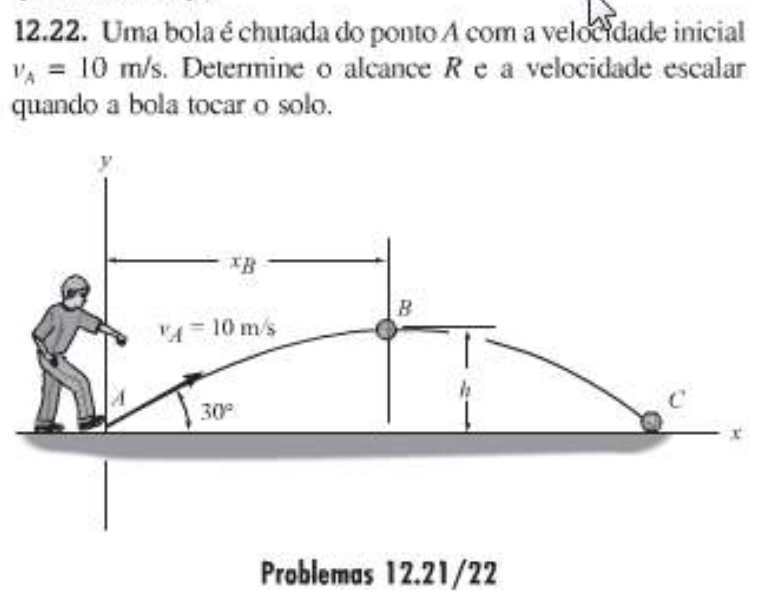
\includegraphics[width=.7\linewidth]{fundamentais/12-22.png}
	\caption{Comando da questão 12-22.}\label{fig?:12-22}
\end{figure}

Nesta questão, analisamos o movimento de um projétil lançado obliquamente com velocidade inicial \(v_A\) e ângulo de lançamento \(\alpha = 30^\circ\). Determinamos o tempo total de voo, o alcance horizontal (\(R\)) e a velocidade escalar no impacto. Também substituímos valores numéricos para ilustrar os resultados.

\subsection*{Componentes da Velocidade Inicial}
As componentes da velocidade inicial são:
\[
v_{Ax} = v_A \cos(\alpha),
\]
\[
v_{Ay} = v_A \sin(\alpha),
\]
onde:
\begin{itemize}
    \item \(v_{Ax}\): Componente horizontal da velocidade;
    \item \(v_{Ay}\): Componente vertical da velocidade.
\end{itemize}

\subsection*{Equações do Movimento}
A aceleração pode ser determinada por
\[
a(t) = \frac{dv}{dt}
\]

E a velocidade é determinada por:
\[
v(t) = \frac{ds}{dt}
\]
Manipulando as equações e combinando-as através de \(dt\), temos:

\[
a\,ds = v\,dv 
\]

Esta equação será a base das análises daqui em diante.

\subsection*{Tempo Total de Voo}

Consideramos que a aceleração horizontal \(a_x = 0\) e a vertical como \(a_y = -g\), o que permite que o alcance \(R\) seja determinado pelo tempo de voo.

O tempo total de voo ocorre quando \(y = 0\). Resolvemos a equação \(y(t) = 0\):
\[
v_{Ay} \cdot t - \frac{1}{2} g t^2 = 0.
\]

Fatorando \(t\), temos:
\[
t \left( v_{Ay} - \frac{1}{2} g t \right) = 0.
\]

A solução positiva é:
\[
t_{\text{total}} = \frac{2 v_{Ay}}{g}.
\]

\subsection*{Alcance Horizontal (\(R\))}
Substituímos \(t_{\text{total}}\) na equação do movimento horizontal para determinar o alcance:
\[
R = x(t_{\text{total}}) = v_{Ax} \cdot t_{\text{total}}.
\]

Substituindo \(t_{\text{total}} = \frac{2 v_{Ay}}{g}\):
\[
R = v_{Ax} \cdot \frac{2 v_{Ay}}{g}.
\]

Usando as expressões para \(v_{Ax}\) e \(v_{Ay}\):
\[
R = \frac{2 v_A^2 \sin(\alpha) \cos(\alpha)}{g}.
\]

Simplificando com a identidade trigonométrica \(\sin(2\alpha) = 2 \sin(\alpha) \cos(\alpha)\):
\[
R = \frac{v_A^2 \sin(2\alpha)}{g}.
\]

\subsection*{Velocidade Escalar no Impacto}
A componente horizontal da velocidade no impacto permanece constante:
\[
v_{x,\text{final}} = v_{Ax}.
\]

A componente vertical no impacto é:
\[
v_{y,\text{final}} = v_{Ay} - g \cdot t_{\text{total}}.
\]

Substituindo \(t_{\text{total}} = \frac{2 v_{Ay}}{g}\):
\[
v_{y,\text{final}} = v_{Ay} - g \cdot \frac{2 v_{Ay}}{g} = -v_{Ay}.
\]

A velocidade escalar no impacto é dada por:
\[
v_{\text{final}} = \sqrt{v_{x,\text{final}}^2 + v_{y,\text{final}}^2}.
\]

Substituindo os valores de \(v_{x,\text{final}}\) e \(v_{y,\text{final}}\):
\[
v_{\text{final}} = \sqrt{v_{Ax}^2 + (-v_{Ay})^2} = \sqrt{v_A^2}. = v_A
\]

\subsection*{Cálculos Numéricos}
Substituímos os seguintes valores:
\[
v_A = 10 \, \text{m/s}, \quad \alpha = 30^\circ = \frac{\pi}{6}, \quad g = 9.81 \, \text{m/s}^2.
\]

O alcance horizontal é:
\[
R = \frac{10^2 \sin(2 \cdot 30^\circ)}{9.81} = \frac{100 \cdot 0.866}{9.81} \approx 8.827 \, \text{m}.
\]

A velocidade escalar no impacto é:
\[
v_{\text{final}} = \sqrt{10^2} = 10 \, \text{m/s}.
\]

\subsection*{Resultados Finais}
\begin{itemize}
    \item Tempo total de voo:
    \[
    t_{\text{total}} = \frac{2 v_A \sin(\alpha)}{g}.
    \]
    \item Alcance horizontal:
    \[
    R = \frac{v_A^2 \sin(2\alpha)}{g} \approx 8.81 \, \text{m}.
    \]
    \item Velocidade escalar no impacto:
    \[
    v_{\text{final}} = v_A = 10 \, \text{m/s}.
    \]
\end{itemize}

	\newpage
\section{Questão 12-23}

\begin{figure}[H]
	\centering
	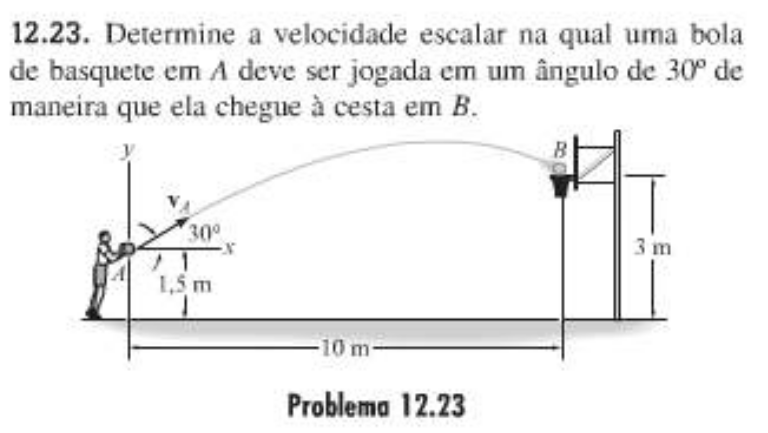
\includegraphics[width=.7\linewidth]{fundamentais/12-23.png}
	\caption{Comando da questão 12-23.}\label{fig:12-23}
\end{figure}

Nesta questão, analisamos o movimento de um projétil lançado de uma altura inicial \(y_0 = 1.5 \, \text{m}\) com um ângulo de lançamento de \(30^\circ\). O projétil percorre uma distância horizontal de \(x = 10 \, \text{m}\) e atinge uma altura final de \(y_f = 3 \, \text{m}\). Nosso objetivo é determinar a velocidade inicial \(v_A\) necessária para satisfazer essas condições.

\subsection*{Equações do Movimento}
As equações do movimento horizontal e vertical são:
\[
x = v_A \cdot \cos(\theta) \cdot t,
\]
\[
y_f = y_0 + v_A \cdot \sin(\theta) \cdot t - \frac{1}{2} g \cdot t^2,
\]
onde:
\begin{itemize}
    \item \(x = 10 \, \text{m}\): Distância horizontal;
    \item \(y_0 = 1.5 \, \text{m}\): Altura inicial;
    \item \(y_f = 3 \, \text{m}\): Altura final;
    \item \(g = 9.81 \, \text{m/s}^2\): Aceleração gravitacional;
    \item \(\theta = 30^\circ = \frac{\pi}{6}\): Ângulo de lançamento.
\end{itemize}

\subsection*{Movimento Horizontal}
Do movimento horizontal, temos:
\[
x = v_A \cdot \cos(\theta) \cdot t.
\]

Resolvendo para o tempo \(t\):
\[
t = \frac{x}{v_A \cdot \cos(\theta)}.
\]

\subsection*{Movimento Vertical}
Substituímos \(t = \frac{x}{v_A \cdot \cos(\theta)}\) na equação do movimento vertical:
\[
y_f = y_0 + v_A \cdot \sin(\theta) \cdot \frac{x}{v_A \cdot \cos(\theta)} - \frac{1}{2} g \cdot \left(\frac{x}{v_A \cdot \cos(\theta)}\right)^2.
\]

Simplificando:
\[
y_f = y_0 + x \cdot \tan(\theta) - \frac{g \cdot x^2}{2 \cdot v_A^2 \cdot \cos^2(\theta)}.
\]

Substituímos \(y_0 = 1.5 \, \text{m}\), \(y_f = 3 \, \text{m}\), \(x = 10 \, \text{m}\), \(g = 9.81 \, \text{m/s}^2\), e \(\cos(30^\circ) = \sqrt{3}/2\), \(\tan(30^\circ) = 1/\sqrt{3}\):
\[
3 = 1.5 + 10 \cdot \frac{1}{\sqrt{3}} - \frac{9.81 \cdot 10^2}{2 \cdot v_A^2 \cdot \left(\frac{\sqrt{3}}{2}\right)^2}.
\]

Simplificando:
\[
3 = 1.5 + \frac{10}{\sqrt{3}} - \frac{9.81 \cdot 100}{v_A^2 \cdot \frac{3}{4}}.
\]

\[
3 = 1.5 + \frac{10}{\sqrt{3}} - \frac{1308}{v_A^2}.
\]

\subsection*{Resolução para \(v_A\)}
Reorganizamos a equação para resolver \(v_A\):
\[
v_A^2 = \frac{1308}{3 - 1.5 - \frac{10}{\sqrt{3}}}.
\]

Calculando:
\[
v_A \approx 12.37 \, \text{m/s}.
\]

\subsection*{Resultado Final}
A velocidade inicial necessária para que o projétil atinja a altura final \(y_f = 3 \, \text{m}\) após percorrer \(x = 10 \, \text{m}\) é:
\[
v_A \approx 12.37 \, \text{m/s}.
\]

	\newpage
\section{Questão 12-27}

\begin{figure}[H]
	\centering
	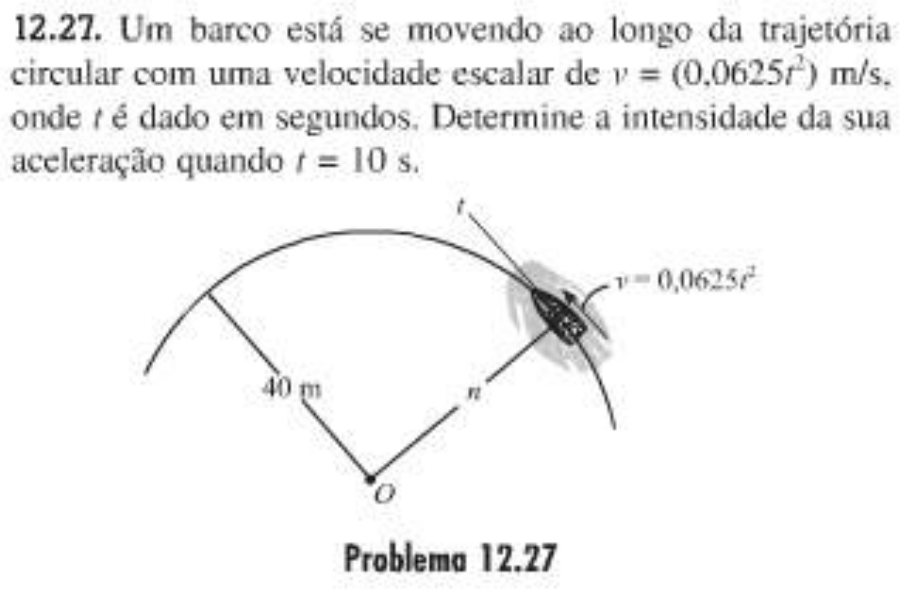
\includegraphics[width=.7\linewidth]{fundamentais/12-27.png}
	\caption{Comando da questão 12-27.}\label{fig:q12-27}
\end{figure}

Nesta questão, analisamos o movimento de uma partícula em uma trajetória circular de raio \(r = 40 \, \text{m}\), cuja velocidade escalar é dada por \(v(t) = 0.0625 \cdot t^2\) (em m/s). Calculamos as acelerações tangencial, centrípeta e total (resultante) e avaliamos seus valores no instante \(t = 10 \, \text{s}\).

\subsection*{Aceleração Tangencial}
A aceleração tangencial é obtida como a derivada da velocidade escalar em relação ao tempo:
\[
a_t = \frac{dv}{dt}.
\]

Derivando \(v(t) = 0.0625 \cdot t^2\):
\[
a_t = \frac{d}{dt}\left(0.0625 \cdot t^2\right) = 0.125 \cdot t.
\]

\subsection*{Aceleração Centrípeta}
A aceleração centrípeta é dada por:
\[
a_c = \frac{v^2}{r}.
\]

Substituímos \(v(t) = 0.0625 \cdot t^2\) e \(r = 40 \, \text{m}\):
\[
a_c = \frac{\left(0.0625 \cdot t^2\right)^2}{40} = \frac{0.00390625 \cdot t^4}{40} = 0.00009765625 \cdot t^4.
\]

\subsection*{Aceleração Total (Resultante)}
A aceleração total é a soma vetorial das componentes tangencial e centrípeta:
\[
a_{\text{total}} = \sqrt{a_t^2 + a_c^2}.
\]

Substituímos \(a_t = 0.125 \cdot t\) e \(a_c = 0.00009765625 \cdot t^4\):
\[
a_{\text{total}} = \sqrt{\left(0.125 \cdot t\right)^2 + \left(0.00009765625 \cdot t^4\right)^2}.
\]

\subsection*{Cálculos no Instante \(t = 10 \, \text{s}\)}
Substituímos \(t = 10 \, \text{s}\) nas expressões para calcular os valores numéricos:
\begin{itemize}
    \item Aceleração tangencial:
    \[
    a_t = 0.125 \cdot 10 = 1.25 \, \text{m/s}^2.
    \]
    \item Aceleração centrípeta:
    \[
    a_c = 0.00009765625 \cdot 10^4 = 0.9765625 \, \text{m/s}^2.
    \]
    \item Aceleração total:
    \[
    a_{\text{total}} = \sqrt{1.25^2 + 0.9765625^2} \approx 1.5862 \, \text{m/s}^2.
    \]
\end{itemize}


	\section{Questão 12-30}

Nesta questão, analisamos o movimento de uma partícula cuja trajetória é descrita por \(y = \frac{1}{8}x^2\). Sabendo que a velocidade escalar é constante (\(v = 6 \, \text{m/s}\)) e que a aceleração tangencial é \(a_t = 1.8 \, \text{m/s}^2\), determinamos o ângulo de inclinação da trajetória (\(\theta\)), a aceleração normal (\(a_n\)) e a aceleração total (\(a_{\text{total}}\)) no ponto \(x = 3 \, \text{m}\).

\subsection*{Equação da Trajetória}
A equação da trajetória é dada por:
\[
y = \frac{1}{8}x^2.
\]

\subsection*{Derivada da Trajetória e Ângulo de Inclinação}
A inclinação da trajetória é obtida pela derivada de \(y\) em relação a \(x\):
\[
\frac{dy}{dx} = \frac{1}{4}x.
\]

O ângulo de inclinação \(\theta\) é dado por:
\[
\theta = \arctan\left(\frac{dy}{dx}\right).
\]

Substituindo \(x = 3 \, \text{m}\):
\[
\theta = \arctan\left(\frac{1}{4} \cdot 3\right) = \arctan\left(\frac{3}{4}\right).
\]

Convertendo para graus:
\[
\theta \approx 36.87^\circ.
\]

\subsection*{Aceleração Normal (\(a_n\))}
A aceleração normal é calculada como:
\[
a_n = \frac{v^2 \cdot \left|\frac{dy}{dx}\right|}{\sqrt{1 + \left(\frac{dy}{dx}\right)^2}}.
\]

Substituímos \(v = 6 \, \text{m/s}\) e \(\frac{dy}{dx} = \frac{1}{4}x\):
\[
a_n = \frac{6^2 \cdot \left|\frac{1}{4}x\right|}{\sqrt{1 + \left(\frac{1}{4}x\right)^2}}.
\]

Para \(x = 3 \, \text{m}\):
\[
a_n = \frac{6^2 \cdot \left|\frac{1}{4} \cdot 3\right|}{\sqrt{1 + \left(\frac{1}{4} \cdot 3\right)^2}} = \frac{36 \cdot \frac{3}{4}}{\sqrt{1 + \left(\frac{3}{4}\right)^2}}.
\]

Simplificando:
\[
a_n \approx 8.57 \, \text{m/s}^2.
\]

\subsection*{Aceleração Total (\(a_{\text{total}}\))}
A aceleração total é a soma vetorial das componentes tangencial e normal:
\[
a_{\text{total}} = \sqrt{a_t^2 + a_n^2}.
\]

Substituímos \(a_t = 1.8 \, \text{m/s}^2\) e \(a_n \approx 8.57 \, \text{m/s}^2\):
\[
a_{\text{total}} = \sqrt{1.8^2 + 8.57^2}.
\]

Simplificando:
\[
a_{\text{total}} \approx 8.76 \, \text{m/s}^2.
\]

\subsection*{Resultados Finais}
\begin{itemize}
    \item Ângulo de inclinação:
    \[
    \theta \approx 36.87^\circ \quad \text{(em \(x = 3 \, \text{m}\))}.
    \]
    \item Aceleração normal:
    \[
    a_n \approx 8.57 \, \text{m/s}^2 \quad \text{(em \(x = 3 \, \text{m}\))}.
    \]
    \item Aceleração total:
    \[
    a_{\text{total}} \approx 8.76 \, \text{m/s}^2 \quad \text{(em \(x = 3 \, \text{m}\))}.
    \]
\end{itemize}

	\section{Questão:12-31}

Nesta questão, analisamos o movimento de uma partícula ao longo de uma curva circular com raio \(r = 300 \, \text{m}\). A aceleração tangencial da partícula é variável e descrita pela equação \(a_t = -0.001 \cdot s\), onde \(s\) é a posição ao longo do arco em metros. Sabemos que a velocidade da partícula no ponto \(A\) (\(s = 0\)) é \(v_A = 25 \, \text{m/s}\). Nosso objetivo é determinar a velocidade da partícula no ponto \(B\) (\(s = r = 300 \, \text{m}\)).

\subsection*{Equação do Movimento}
A equação do movimento é dada por:
\[
a_t = v \cdot \frac{dv}{ds},
\]
onde:
\begin{itemize}
    \item \(a_t = -0.001 \cdot s\): Aceleração tangencial variável;
    \item \(v\): Velocidade escalar da partícula;
    \item \(s\): Posição ao longo do arco.
\end{itemize}

Substituímos \(a_t\) na equação:
\[
-0.001 \cdot s = v \cdot \frac{dv}{ds}.
\]

Reorganizando:
\[
v \cdot dv = -0.001 \cdot s \cdot ds.
\]

\subsection*{Integração}
Integramos ambos os lados para determinar \(v\) em função de \(s\). No ponto \(A\), temos \(v = v_A = 25 \, \text{m/s}\) quando \(s = 0\):
\[
\int_{v_A}^{v} v \, dv = \int_{0}^{s} -0.001 \cdot s \, ds.
\]

Resolvendo a integral do lado esquerdo:
\[
\frac{v^2}{2} \bigg|_{v_A}^{v} = -0.001 \cdot \frac{s^2}{2} \bigg|_{0}^{s}.
\]

Substituímos os limites:
\[
\frac{v^2}{2} - \frac{v_A^2}{2} = -0.001 \cdot \frac{s^2}{2}.
\]

Reorganizando para \(v^2\):
\[
v^2 = v_A^2 - 0.001 \cdot s^2.
\]

\subsection*{Velocidade no Ponto \(B\)}
No ponto \(B\), \(s = r = 300 \, \text{m}\). Substituímos \(s = 300 \, \text{m}\) e \(v_A = 25 \, \text{m/s}\) na equação:
\[
v^2 = 25^2 - 0.001 \cdot (300)^2.
\]

Calculando:
\[
v^2 = 625 - 0.001 \cdot 90000.
\]

\[
v^2 = 625 - 90 = 535.
\]

A velocidade no ponto \(B\) é:
\[
v = \sqrt{535} \approx 23.13 \, \text{m/s}.
\]

\subsection*{Resultado Final}
A velocidade da partícula no ponto \(B\) (\(s = r = 300 \, \text{m}\)) é:
\[
v \approx 23.13 \, \text{m/s}.
\]

	\newpage
\section{Questão 12-33}

\begin{figure}[H]
	\centering
	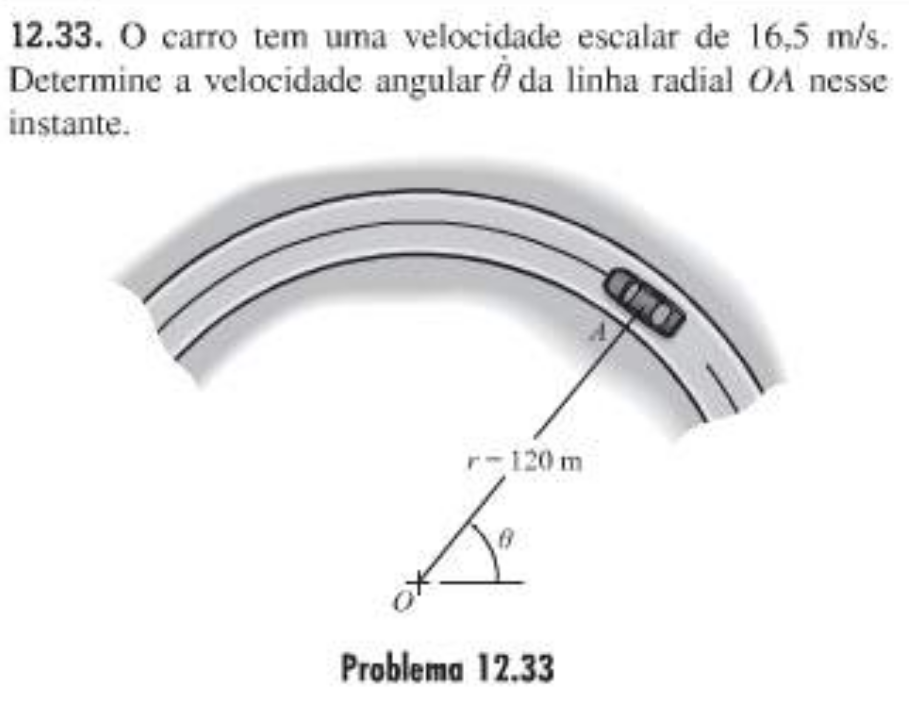
\includegraphics[width=.7\linewidth]{fundamentais/12-33.png}
	\caption{Comando da questão 12-33}\label{fig:12-33}
\end{figure}

Nesta questão, analisamos o movimento de uma partícula em uma trajetória circular com raio \(r = 120 \, \text{m}\) e velocidade escalar \(v = 16.5 \, \text{m/s}\). Determinamos a velocidade angular \(\dot{\theta}\) da partícula.

\subsection*{Cálculo da Velocidade Angular}
A relação entre a velocidade angular \(\dot{\theta}\) e a velocidade escalar \(v\) em uma trajetória circular é dada por:
\[
\dot{\theta} = \frac{v}{r},
\]
onde:
\begin{itemize}
    \item \(\dot{\theta}\): Velocidade angular (em rad/s);
    \item \(v\): Velocidade escalar (em m/s);
    \item \(r\): Raio da trajetória circular (em m).
\end{itemize}

\subsection*{Substituição dos Valores Numéricos}
Substituímos os valores \(v = 16.5 \, \text{m/s}\) e \(r = 120 \, \text{m}\) na equação:
\[
\dot{\theta} = \frac{16.5}{120}.
\]

Simplificando:
\[
\dot{\theta} \approx 0.138 \, \text{rad/s}.
\]

\subsection*{Resultado Final}
A velocidade angular da partícula é:
\[
\dot{\theta} \approx 0.138 \, \text{rad/s}.
\]

	\section{Questão 12-34}

Nesta questão, analisamos o movimento de uma partícula em coordenadas polares, onde a posição radial e a posição angular variam com o tempo. A posição radial é dada por \(r(t) = 0.1 \cdot t^3\), e a posição angular é \( \theta(t) = 4 \cdot t^{3/2}\). Calculamos as velocidades, acelerações e suas intensidades no instante \(t = 1.5 \, \text{s}\).

\subsection*{Velocidade Radial e Angular}
A velocidade radial é a derivada de \(r(t)\) em relação ao tempo:
\[
\frac{dr}{dt} = \frac{d}{dt}\left(0.1 \cdot t^3\right) = 0.3 \cdot t^2.
\]

A velocidade angular é a derivada de \(\theta(t)\) em relação ao tempo:
\[
\frac{d\theta}{dt} = \frac{d}{dt}\left(4 \cdot t^{3/2}\right) = 6 \cdot t^{1/2}.
\]

\subsection*{Velocidade Tangencial e Intensidade da Velocidade Total}
A velocidade tangencial é dada por:
\[
v_{\text{tangencial}} = r \cdot \frac{d\theta}{dt}.
\]

Substituímos \(r(t) = 0.1 \cdot t^3\) e \(\frac{d\theta}{dt} = 6 \cdot t^{1/2}\):
\[
v_{\text{tangencial}} = \left(0.1 \cdot t^3\right) \cdot \left(6 \cdot t^{1/2}\right) = 0.6 \cdot t^{7/2}.
\]

A intensidade da velocidade total é:
\[
v_{\text{total}} = \sqrt{\left(\frac{dr}{dt}\right)^2 + v_{\text{tangencial}}^2}.
\]

Substituímos \(\frac{dr}{dt} = 0.3 \cdot t^2\) e \(v_{\text{tangencial}} = 0.6 \cdot t^{7/2}\):
\[
v_{\text{total}} = \sqrt{\left(0.3 \cdot t^2\right)^2 + \left(0.6 \cdot t^{7/2}\right)^2}.
\]

\subsection*{Acelerações Radial e Tangencial}
A aceleração radial (centrípeta) é dada por:
\[
a_{\text{radial}} = r \cdot \left(\frac{d\theta}{dt}\right)^2.
\]

Substituímos \(r(t) = 0.1 \cdot t^3\) e \(\frac{d\theta}{dt} = 6 \cdot t^{1/2}\):
\[
a_{\text{radial}} = \left(0.1 \cdot t^3\right) \cdot \left(6 \cdot t^{1/2}\right)^2 = 3.6 \cdot t^{4}.
\]

A aceleração tangencial é a derivada de \(v_{\text{tangencial}}\) em relação ao tempo:
\[
a_{\text{tangencial}} = \frac{d}{dt}\left(0.6 \cdot t^{7/2}\right) = 2.1 \cdot t^{5/2}.
\]

A intensidade da aceleração total é:
\[
a_{\text{total}} = \sqrt{a_{\text{radial}}^2 + a_{\text{tangencial}}^2}.
\]

Substituímos \(a_{\text{radial}} = 3.6 \cdot t^4\) e \(a_{\text{tangencial}} = 2.1 \cdot t^{5/2}\):
\[
a_{\text{total}} = \sqrt{\left(3.6 \cdot t^4\right)^2 + \left(2.1 \cdot t^{5/2}\right)^2}.
\]

\subsection*{Cálculos no Instante \(t = 1.5 \, \text{s}\)}
Substituímos \(t = 1.5 \, \text{s}\) nas expressões:
\begin{itemize}
    \item Velocidade total:
    \[
    v_{\text{total}} = \sqrt{\left(0.3 \cdot 1.5^2\right)^2 + \left(0.6 \cdot 1.5^{7/2}\right)^2} \approx 3.813 \, \text{m/s}.
    \]
    \item Aceleração total:
    \[
    a_{\text{total}} = \sqrt{\left(3.6 \cdot 1.5^4\right)^2 + \left(2.1 \cdot 1.5^{5/2}\right)^2} \approx 36.419 \, \text{m/s}^2.
    \]
\end{itemize}

\subsection*{Resultados Finais}
\begin{itemize}
    \item Intensidade da velocidade total:
    \[
    v_{\text{total}} \approx 3.813 \, \text{m/s}.
    \]
    \item Intensidade da aceleração total:
    \[
    a_{\text{total}} \approx 36.419 \, \text{m/s}^2.
    \]
\end{itemize}

	\section{Questão 12-39}

Nesta questão, analisamos um sistema de polias em que a velocidade de um ponto \(A\) é relacionada à velocidade de um bloco \(D\) devido à configuração do sistema de cordas. Determinamos a velocidade de \(D\) (\(v_D\)) quando a velocidade de \(A\) (\(v_A\)) é \(3 \, \text{m/s}\).

\subsection*{Relação entre as Velocidades}
No sistema de polias, a velocidade de \(A\) é o dobro da velocidade de \(D\), pois a corda se divide em duas partes móveis conectadas ao bloco \(D\). Assim, temos a relação:
\[
v_A = 2 \cdot v_D,
\]
onde:
\begin{itemize}
    \item \(v_A\): Velocidade no ponto \(A\);
    \item \(v_D\): Velocidade no bloco \(D\).
\end{itemize}

\subsection*{Cálculo de \(v_D\)}
Substituímos \(v_A = 3 \, \text{m/s}\) na equação:
\[
3 = 2 \cdot v_D.
\]

Resolvendo para \(v_D\):
\[
v_D = \frac{3}{2} = 1.5 \, \text{m/s}.
\]

\subsection*{Resultado Final}
A velocidade do bloco \(D\) é:
\[
v_D = 1.5 \, \text{m/s}.
\]

	\section{Questão 12-40}

Nesta questão, analisamos um sistema de polias em que a velocidade no ponto \(B\) é relacionada à velocidade do bloco \(A\) devido à configuração do sistema de cordas. Determinamos a velocidade de \(A\) (\(v_A\)) quando a velocidade de \(B\) (\(v_B\)) é \(6 \, \text{m/s}\).

\subsection*{Relação entre as Velocidades}
No sistema de polias, a velocidade no ponto \(B\) é o dobro da velocidade do bloco \(A\), pois a corda se divide em duas partes móveis conectadas ao bloco \(A\). Assim, temos a relação:
\[
v_B = 2 \cdot v_A,
\]
onde:
\begin{itemize}
    \item \(v_B\): Velocidade no ponto \(B\);
    \item \(v_A\): Velocidade no bloco \(A\).
\end{itemize}

\subsection*{Cálculo de \(v_A\)}
Substituímos \(v_B = 6 \, \text{m/s}\) na equação:
\[
6 = 2 \cdot v_A.
\]

Resolvendo para \(v_A\):
\[
v_A = \frac{6}{2} = 3 \, \text{m/s}.
\]

\subsection*{Resultado Final}
A velocidade do bloco \(A\) é:
\[
v_A = 3 \, \text{m/s}.
\]

	\section{Questão 12-47}

Nesta questão, analisamos o movimento de dois barcos, \(A\) e \(B\), que se movem em direções diferentes. O barco \(A\) se move com uma velocidade escalar \(v_A = 15 \, \text{m/s}\) a um ângulo de \(30^\circ\) em relação ao eixo \(x\), enquanto o barco \(B\) se move com uma velocidade escalar \(v_B = 10 \, \text{m/s}\) na direção do eixo \(y\). Determinamos a distância entre os barcos no instante \(t = 4 \, \text{s}\).

\subsection*{Posições dos Barcos}
A posição do barco \(A\) é dada por suas componentes \(x_A\) e \(y_A\):
\[
x_A = v_A \cdot t \cdot \cos(\theta),
\]
\[
y_A = v_A \cdot t \cdot \sin(\theta),
\]
onde:
\begin{itemize}
    \item \(v_A = 15 \, \text{m/s}\) é a velocidade escalar do barco \(A\);
    \item \(\theta = 30^\circ = \frac{\pi}{6}\) é o ângulo do movimento do barco \(A\).
\end{itemize}

A posição do barco \(B\) é:
\[
x_B = 0, \quad y_B = v_B \cdot t,
\]
onde \(v_B = 10 \, \text{m/s}\) é a velocidade escalar do barco \(B\).

\subsection*{Distância entre os Barcos}
A distância entre os barcos é dada por:
\[
d(t) = \sqrt{(x_A - x_B)^2 + (y_A - y_B)^2}.
\]

Substituímos as expressões para \(x_A\), \(x_B\), \(y_A\) e \(y_B\):
\[
d(t) = \sqrt{\left(v_A \cdot t \cdot \cos(\theta) - 0\right)^2 + \left(v_A \cdot t \cdot \sin(\theta) - v_B \cdot t\right)^2}.
\]

Simplificando:
\[
d(t) = \sqrt{\left(15 \cdot t \cdot \cos\left(\frac{\pi}{6}\right)\right)^2 + \left(15 \cdot t \cdot \sin\left(\frac{\pi}{6}\right) - 10 \cdot t\right)^2}.
\]

\subsection*{Cálculo para \(t = 4 \, \text{s}\)}
Substituímos \(t = 4 \, \text{s}\) na expressão:
\[
d(4) = \sqrt{\left(15 \cdot 4 \cdot \cos\left(\frac{\pi}{6}\right)\right)^2 + \left(15 \cdot 4 \cdot \sin\left(\frac{\pi}{6}\right) - 10 \cdot 4\right)^2}.
\]

Calculando:
\[
\cos\left(\frac{\pi}{6}\right) = \frac{\sqrt{3}}{2}, \quad \sin\left(\frac{\pi}{6}\right) = \frac{1}{2}.
\]

Substituímos:
\[
d(4) = \sqrt{\left(15 \cdot 4 \cdot \frac{\sqrt{3}}{2}\right)^2 + \left(15 \cdot 4 \cdot \frac{1}{2} - 10 \cdot 4\right)^2}.
\]

Simplificando:
\[
d(4) = \sqrt{\left(60 \cdot \frac{\sqrt{3}}{2}\right)^2 + \left(30 - 40\right)^2},
\]
\[
d(4) = \sqrt{\left(30\sqrt{3}\right)^2 + (-10)^2}.
\]

Calculando:
\[
d(4) = \sqrt{2700 + 100} = \sqrt{2800} \approx 52.92 \, \text{m}.
\]

\subsection*{Resultado Final}
A distância entre os barcos no instante \(t = 4 \, \text{s}\) é:
\[
d(4) \approx 52.92 \, \text{m}.
\]


	% SECÇÃO PROBLEMAS


\end{document}
